\section{Informazioni Generali}

\begin{itemize}
\item{\textbf{Luogo}}: Meeting Google Meet
\item{\textbf{Data}}: \D{}
\item{\textbf{Ora}}: 18:00 - 19:00
\item{\textbf{Partecipanti dell'azienda Zero12}}: 
	\begin{itemize}
	\item{Michele Massaro,} 
	\item{Stefano Dindo.}
	\end{itemize} 
\item{\textbf{Partecipanti del Gruppo}}: 
	\begin{itemize}
	\item{\EP{},} 
	\item{\FP{},}
	\item{\GC{},}
	\item{\LW{},}	
	\item{\MB{},}
	\item{\PV{}.}
	\end{itemize} 
\item{\textbf{Segretario}}: \GC{}
\end{itemize}

\section{Motivo della riunione}
\begin{itemize}
\item{Diagrammi UML e Requisiti}
\item{Discussione su API Gateway}
\item{Discussione sulle Lambda}
\item{Difficoltà Riscontrate con il Crawler TikTok}
\item{Crediti AWS}
\end{itemize}

\section{Resoconto}

\subsection{Diagrammi UML e Requisiti}

La prima cosa che abbiamo mostrato all'azienda in questa riunione esterna sono stati i casi d'uso, i diagrammi UML ed i requisiti presenti nel documento “\textit{Analisi dei Requisiti}”. In particolare, ci siamo soffermati sui casi principali:

\begin{enumerate}
\item Area personale e sottocasi (UCW4 \S{}3.5),
\item Visualizza classifica (UCW7 \S{}3.8),
\item Filtra classifica e sottocasi (UCW8 \S{}3.9),
\item Modifica parametri di ordinamento classifica e sottocasi (UCW9 \S{3.10}).
\end{enumerate}

Poiché abbiamo discusso internamente di alcuni sottocasi del caso d'uso UCW7, abbiamo esposto le nostre perplessità all'azienda, che ci ha dato delle dritte in merito: i nostri dubbi erano relativi a “Filtra per tipo di cucina” (UCW8.3 \S{}3.9.3) e “Filtra per fascia di prezzo” (UCW8.4 \S{}3.9.4), perché non avevamo trovato informazioni necessarie per realizzare questi filtri. Stefano Dindo di Zero 12 ci ha suggerito di risolvere sfruttando i dati raccolti con i servizi Amazon (quali: \textbf{Rekognition} e \textbf{Comprehend}), dopo aver analizzato i contenuti multimediali, realizzando così una soluzione “in casa”.
\\
Per quanto riguarda i restanti casi d'uso, a detta dell'azienda vanno bene.
\\ \\
Lato requisiti, non ci sono stati particolari problemi, ma abbiamo chiesto qualche consiglio in merito alle versioni dei browser su cui dovrà funzionare la piattaforma: l'azienda ha espresso che non è necessario avere una WebApp che sia retrocompatibile, questa non è l'esigenza principale, e quindi vanno bene anche le ultime versioni. Sempre per quanto riguarda i requisiti, abbiamo parlato anche delle API Gateway, di cui parleremo nel prossimo paragrafo, perché non ci erano molto chiare e, soprattutto, non avevamo ben capito il loro ruolo all'interno del progetto.

\subsection{Discussione su API Gateway}

Non ci era molto chiaro cosa fossero le \textbf{API Gateway}; l'azienda ci ha spiegato che è un servizio offerto da Amazon e permette di accedere ai dati presenti nel database, mediante la parte front-end, mantenendo intatta la loro sicurezza: in pratica, è una sorta di interfaccia, che interagisce tra database ed interazioni dell'utente (e, di conseguenza, mostra all'utente ciò che chiede).

\begin{figure}[!h]
\centering
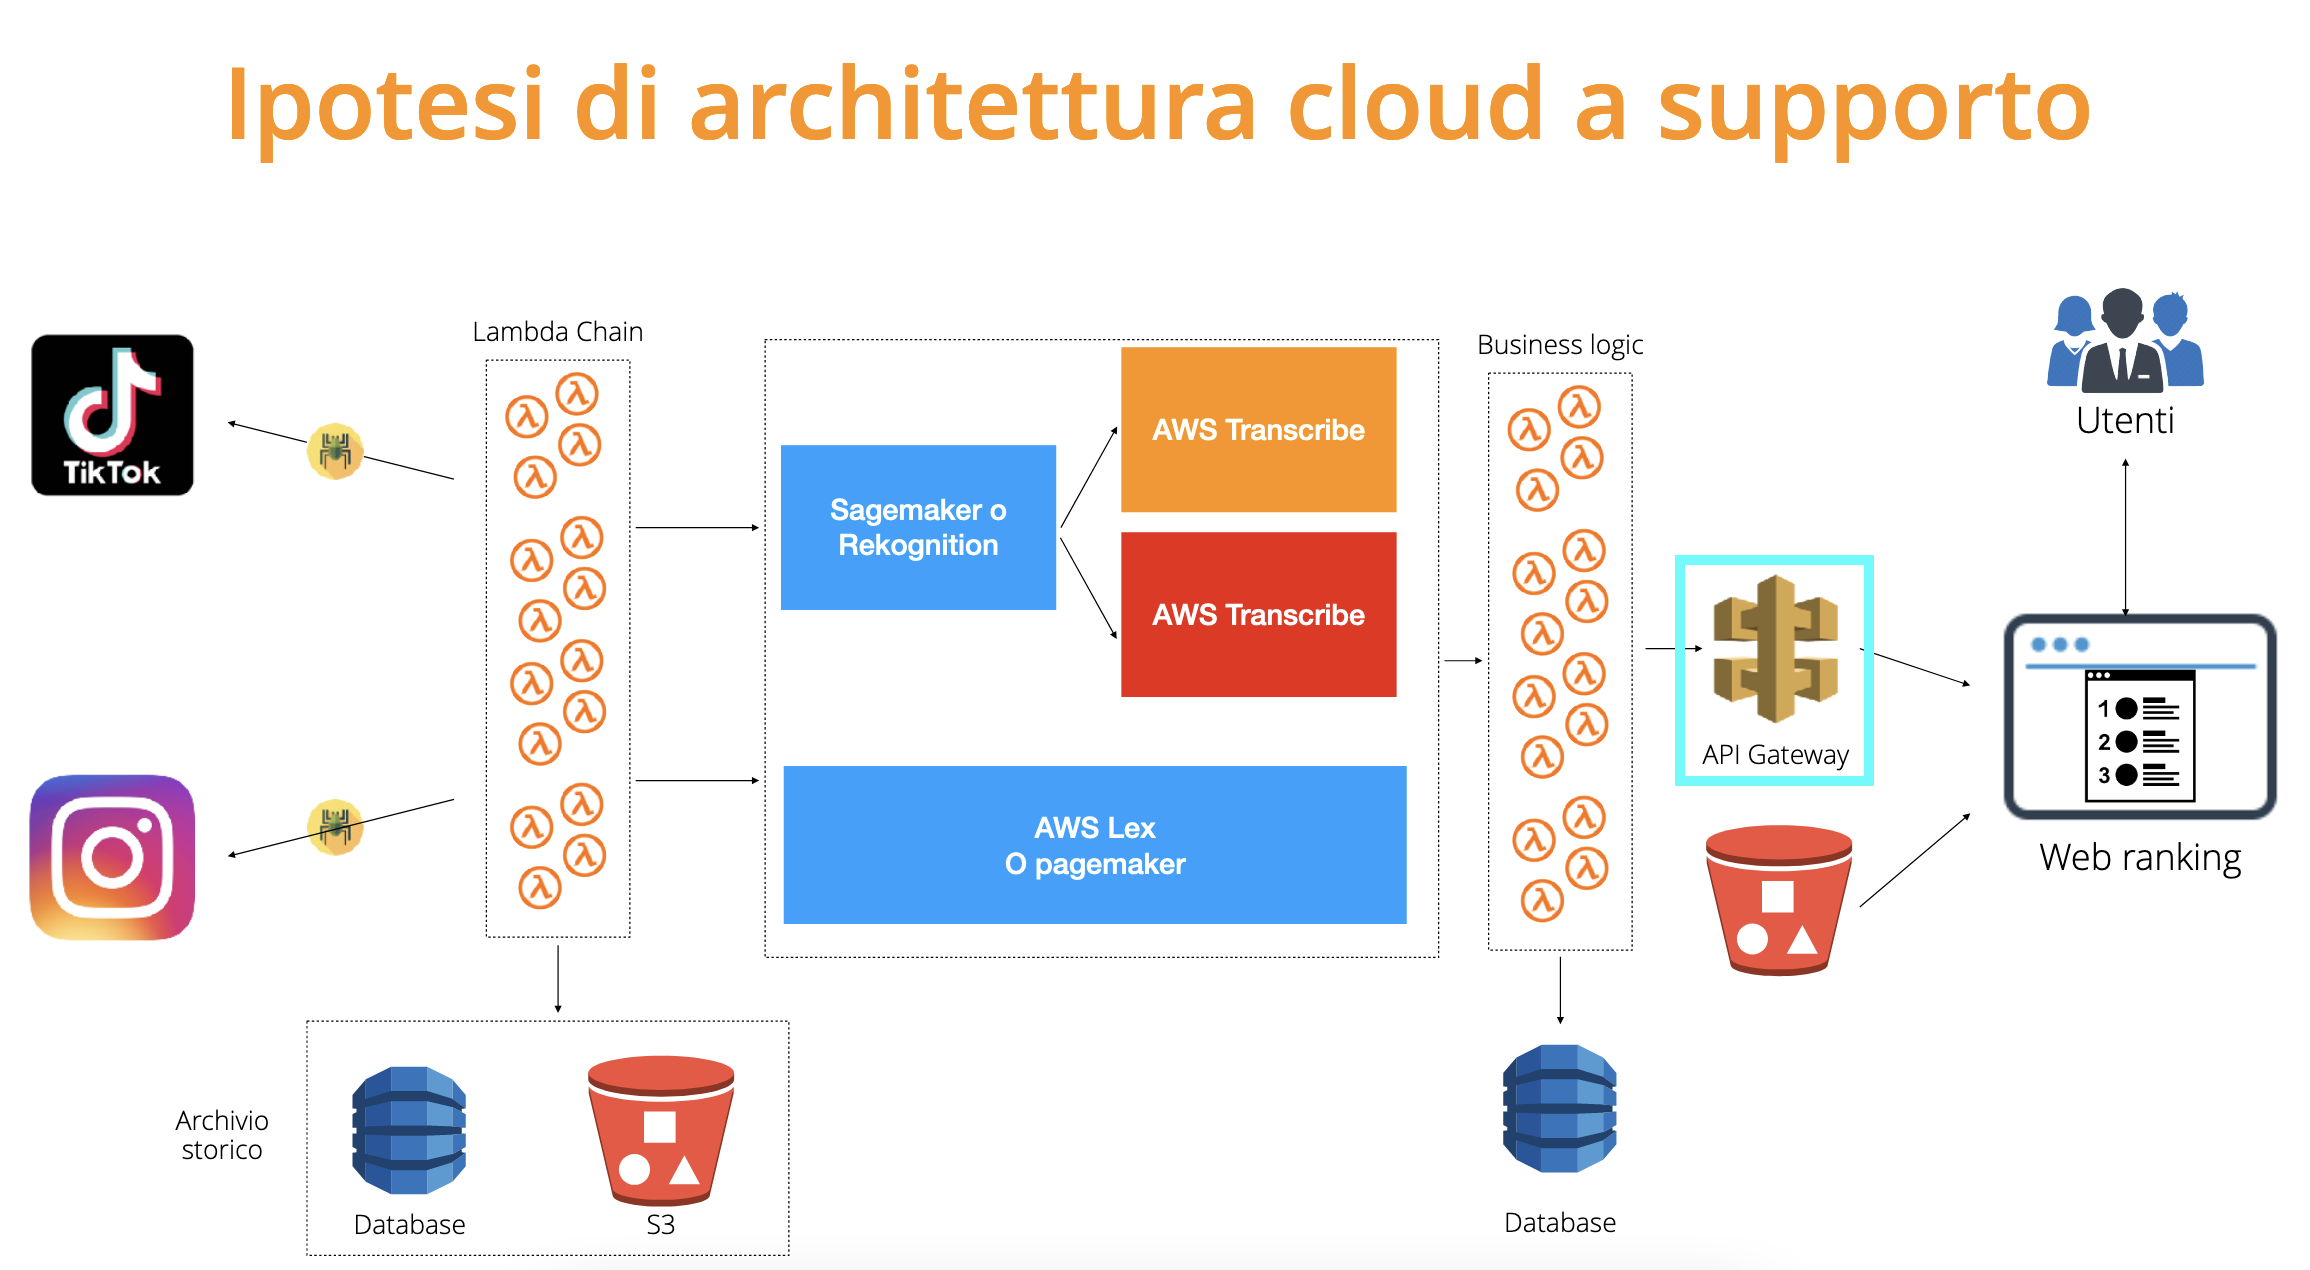
\includegraphics[scale=0.35]{Sezioni/images/Architettura.png}
\caption{Architettura Cloud con evidenziata la parte dove servono le API Gateway}
\end{figure}

\subsection{Discussione sulle Lambda}

Abbiamo illustrato a Zero 12 alcuni dubbi sul corretto utilizzo delle lambda, in particolare non ci era molto chiaro se si dovessero effettuare all'interno della lambda le query di inserimento nel database. L'azienda ci ha risposto che è corretto connettersi al database ed effettuare query all'interno di una lambda.

\subsection{Problemi legati ai crawler}

Sono stati esposti all'azienda alcuni problemi problemi relativi alla poca affidabilità dei crawler i quali potrebbero non funzionare a seguito di un aggiornamento di instagram o di tiktok. Zero 12 ci ha detto che aveva già previsto questo rischio e ci ha suggerito di registrare un video che illustra il funzionamento dei crawler in modo da poterlo avere a disposizione in caso il crawler non funzioni a ridosso di una consegna.  

\subsection{Crediti AWS}

Attualmente stiamo facendo delle prove su un database RDS e stiamo sfruttando i servizi di AWS (quali Rekognition e Comprehend) in versione di test (quindi, gratuitamente), perché non ci sono ancora stati dati i crediti da parte dell'azienda. Zero 12 ha confermato che i crediti dovrebbero arrivare entro la prossima settimana e che il tetto massimo spendibile è di \textbf{2000\$}.

